\documentclass[11pt,a4paper]{article}

% ---------------------------------------------------------------------------
% Packages
% ---------------------------------------------------------------------------
\usepackage[margin=2.3cm]{geometry}
\usepackage[T1]{fontenc}
\usepackage[utf8]{inputenc}
\usepackage{lmodern}
\usepackage{microtype}
\usepackage{graphicx}
\usepackage{booktabs}
\usepackage{longtable}
\usepackage[table]{xcolor}
\usepackage{amsmath}
\usepackage{caption}
\usepackage{subcaption}
\usepackage{float}
\usepackage{enumitem}
\usepackage{multirow}
\usepackage[colorlinks=true,linkcolor=blue!50!black,urlcolor=blue!50!black,citecolor=blue!50!black]{hyperref}

\graphicspath{{figures/}}
\captionsetup{font=small,labelfont=bf}
\setlist{itemsep=2pt,topsep=4pt}
\setlength{\parskip}{4pt}

% Red notes for the team: remove them all before submitting
\newcommand{\todo}[1]{\textcolor{red}{\textbf{[TO DO: #1]}}}

% ---------------------------------------------------------------------------
\begin{document}

\begin{center}
  {\LARGE \textbf{Predicting High Income from Census Data}}\\[4pt]
  {\large An end-to-end supervised learning proof-of-concept}\\[10pt]
  \textbf{Dataset: Option 1 -- Adult / Census Income} (OpenML \texttt{adult}, version 2)\\[6pt]
  Alexandre Casagranda, Simon Mazabraud, Ryan Khlaief\\[2pt]
  Applied ML: Foundations, Engineering \& Evaluation (MSA-DATI07-05) -- Albert School\\[2pt]
  GitHub repository: \url{https://github.com/acasagranda24/Applied-ML-project}\\[2pt]
  November 2026
\end{center}

\begin{abstract}
\noindent We predict whether an adult earns more than \$50K per year from the 1994 US census (48{,}842 people, 23.9\% positives).
All decisions are taken with 5-fold stratified cross-validation on an 80\% development set, and a 20\% test set is used only once at the end.
We compare four models of increasing flexibility: logistic regression, a decision tree, a random forest and LightGBM.
After tuning with Optuna, LightGBM is the best model (cross-validated PR-AUC $0.830 \pm 0.007$).
On the test set it reaches a PR-AUC of 0.837 and, with a decision threshold of 0.379 tuned on out-of-fold predictions, an F1 score of 0.728.
Its probabilities are well calibrated (Brier score 0.086, ECE 0.007).
SHAP shows that the model mainly uses capital income, age, marital status and education, which makes business sense.
Finally, a fairness audit by sex shows a recall gap of 7.5 points between men and women.
Group-specific decision thresholds close this gap: after mitigation it is no longer statistically distinguishable from zero, with almost no loss in overall performance.
\end{abstract}

% ===========================================================================
\section{Problem framing}
\label{sec:framing}

\paragraph{Business question.}
Imagine a bank or a public agency that wants to target a product or a policy at people with a high income, but does not know their income.
Our model must answer one question for each person: \emph{does this person earn more than \$50K per year?}
This is a binary classification task. The positive class (\texttt{>50K}) is the minority class.

\paragraph{The five framing questions.}
\begin{itemize}
  \item \textbf{Unit of decision:} one adult from the census.
  \item \textbf{Target:} income above \$50K per year (1) or not (0).
  \item \textbf{Leakage audit:} all features describe the person (age, education, job, family situation, hours worked, capital income). They are known before the income and none of them is computed from the target. We found no leaking feature.
  \item \textbf{Split:} stratified 80/20 development/test split, with 5-fold cross-validation inside the development set (Section~\ref{sec:protocol}).
  \item \textbf{No-skill baseline:} a dummy classifier that always predicts the class frequencies. Its PR-AUC equals the positive rate (0.239). Every real model must beat it.
\end{itemize}

\paragraph{Sensitive attribute.}
The dataset contains \texttt{sex} and \texttt{race}. We use \texttt{sex} as the main sensitive attribute for the fairness audit (Section~\ref{sec:fairness}). Some race groups are very small (less than 1\% of the data), so their metrics would be too noisy.

% ===========================================================================
\section{Exploratory data analysis}
\label{sec:eda}

The dataset has 48{,}842 rows and 14 features (6 numeric, 8 categorical). Table~\ref{tab:eda} summarises the main findings. Each finding led to a decision that we implemented in the code (\texttt{src/eda.py} prints them all).

\begin{table}[!htbp]
\centering
\small
\caption{Main findings of the EDA and the decisions they led to.}
\label{tab:eda}
\begin{tabular}{p{7.2cm}p{7.6cm}}
\toprule
\textbf{Finding} & \textbf{Decision} \\
\midrule
76.1\% \texttt{<=50K} vs 23.9\% \texttt{>50K}. Always predicting \texttt{<=50K} gives 76\% accuracy. & Accuracy is misleading. PR-AUC is our main metric (Section~\ref{sec:imbalance}). \\
\addlinespace
\texttt{workclass} (5.7\%), \texttt{occupation} (5.8\%) and \texttt{native-country} (1.8\%) have missing values. The same 2{,}799 people miss both \texttt{workclass} and \texttt{occupation}, and only 9.4\% of them earn \texttt{>50K} (vs 24.8\%). & Missing values are \emph{not random}: we keep them as an explicit \texttt{"Missing"} category instead of dropping rows or using the most frequent value. \\
\addlinespace
\texttt{capital-gain} and \texttt{capital-loss} are 91.7\% and 95.3\% zeros, with a very long tail (max 99{,}999). & New features \texttt{capital\_net} (signed log) and \texttt{has\_capital} (flag). \\
\addlinespace
46.7\% of people work exactly 40 hours per week. & New flag \texttt{overtime} (more than 40 hours). \\
\addlinespace
\texttt{native-country} has 41 values, but 91.3\% are United-States. & New flag \texttt{native\_us} instead of 41 sparse one-hot columns. \\
\addlinespace
\texttt{education} (16 text values) maps one-to-one to \texttt{education-num}. & Drop \texttt{education}, keep the ordinal \texttt{education-num}. \\
\addlinespace
\texttt{fnlwgt} is a census sampling weight (how many people a row represents), with the same distribution in both classes. & Drop \texttt{fnlwgt}: it is not a property of the person. \\
\addlinespace
52 exact duplicate rows (0.1\%). & Keep them: two people can share the same attributes. \\
\addlinespace
30.4\% of men vs 10.9\% of women earn \texttt{>50K}. Women are 33\% of the rows. & Large base-rate gap: this motivates the fairness audit. \\
\bottomrule
\end{tabular}
\end{table}

Figure~\ref{fig:eda} shows the share of high earners in each category. Marital status and relationship are the strongest signals: married people (husbands and wives) earn more than \$50K much more often than the others.
Note that \texttt{relationship} (\emph{Husband}/\emph{Wife}) is almost a copy of \texttt{sex}. This matters for fairness: removing \texttt{sex} from the features would not make the model blind to it.

\begin{figure}[!htbp]
  \centering
  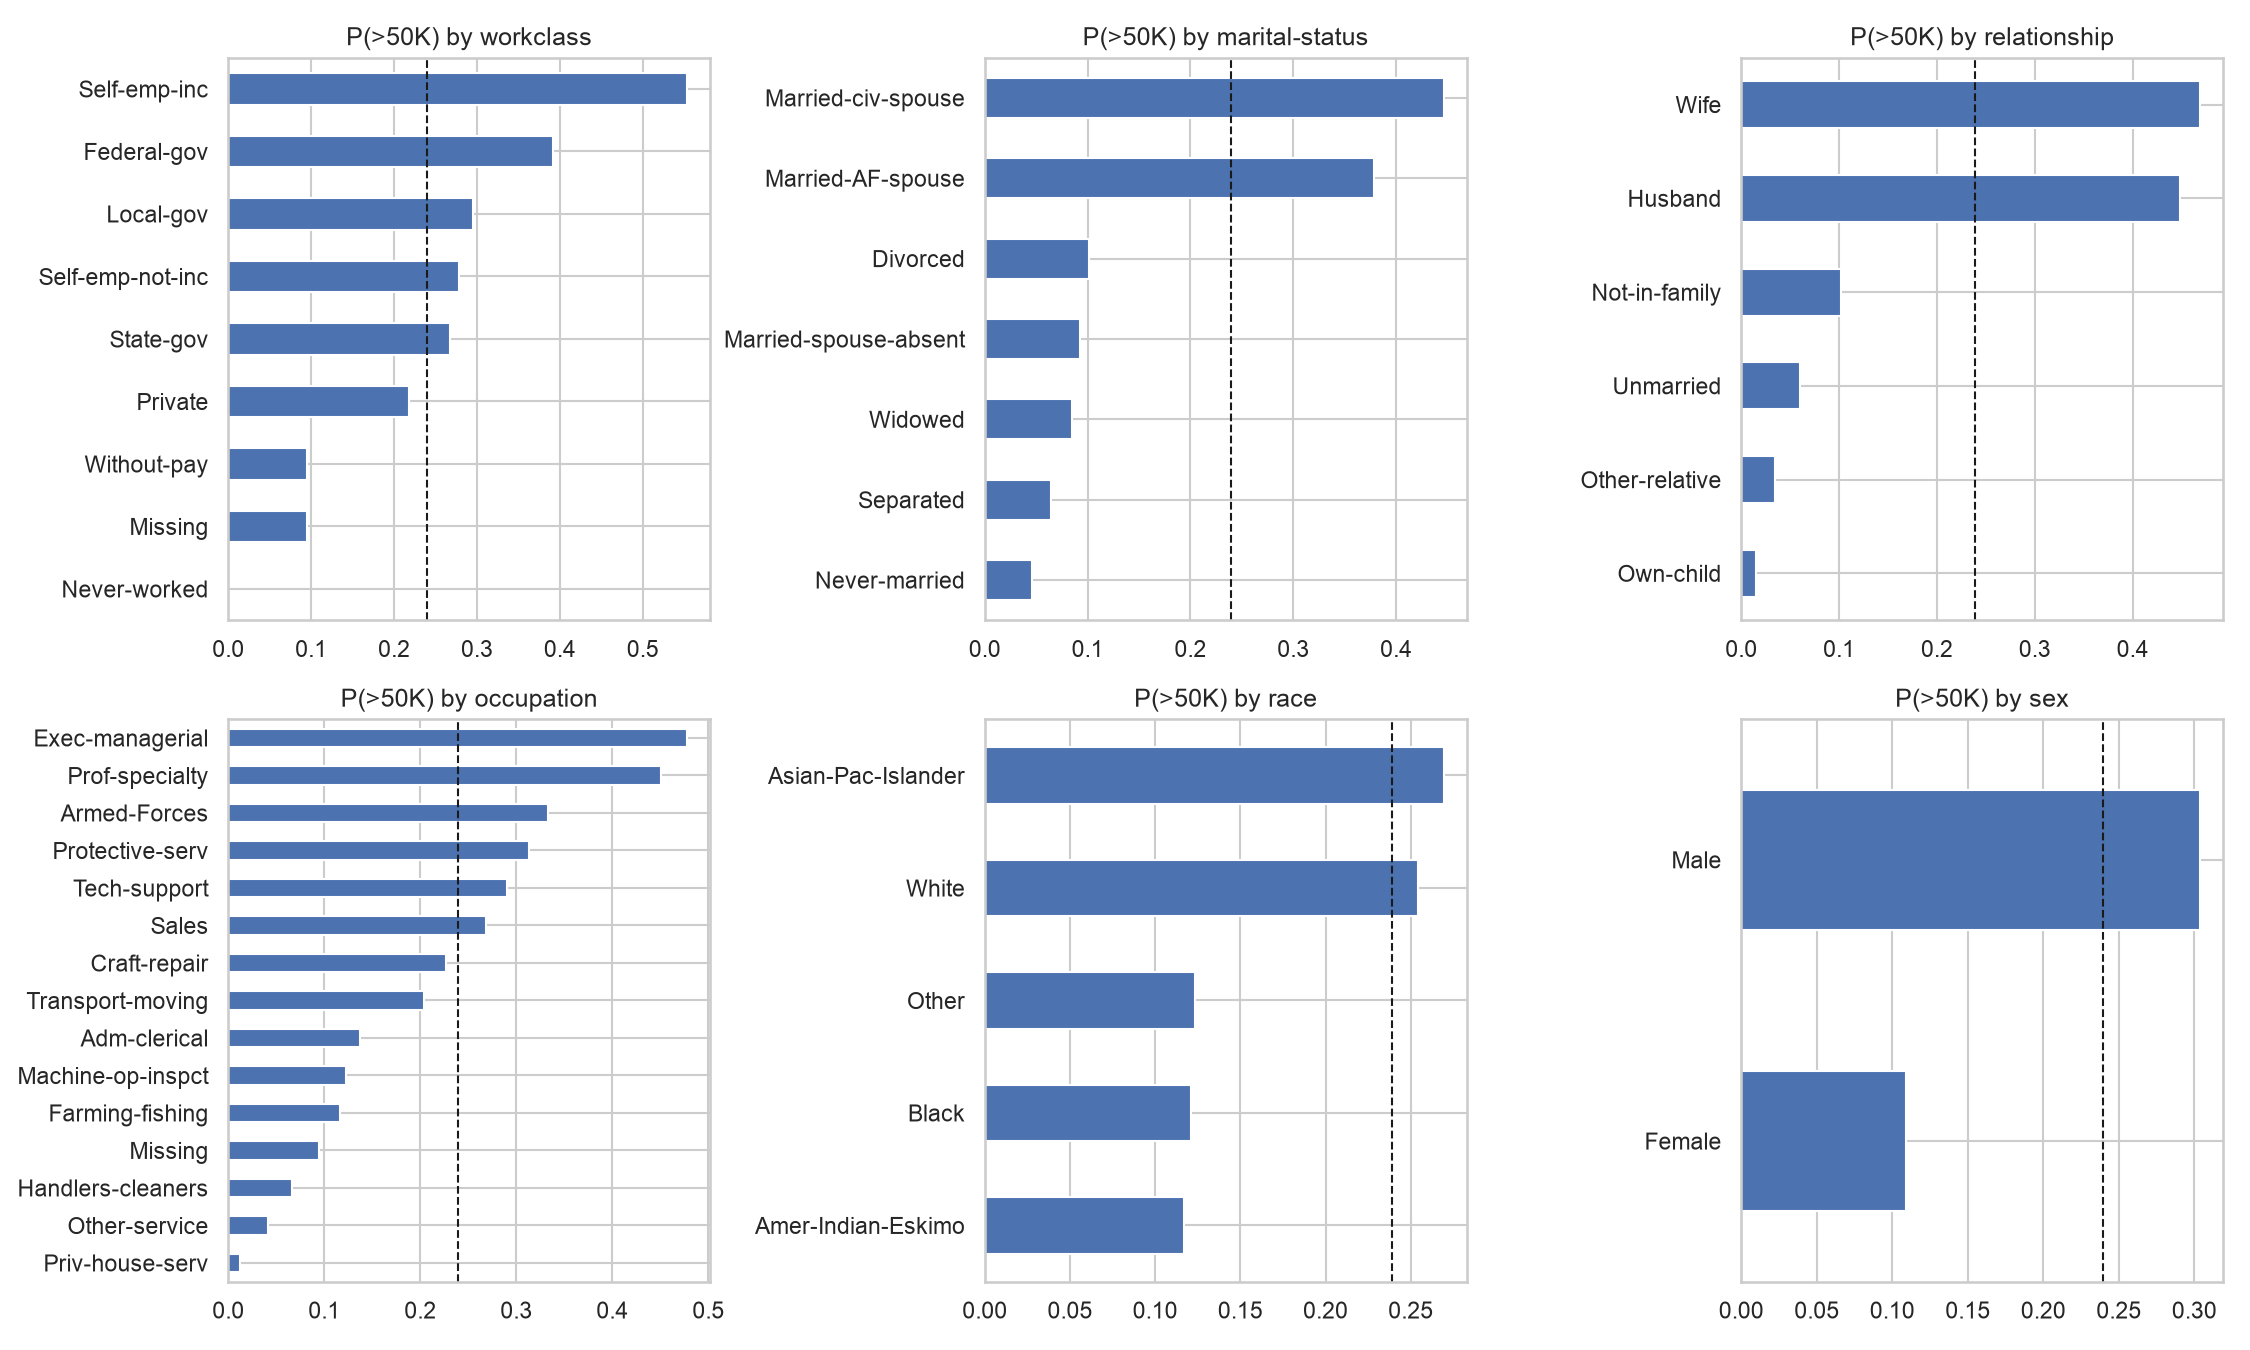
\includegraphics[width=\textwidth]{eda_positive_rate_by_category.png}
  \caption{Share of people earning \texttt{>50K} in each category. The dashed line is the global rate (23.9\%).}
  \label{fig:eda}
\end{figure}

% ===========================================================================
\section{Validation protocol}
\label{sec:protocol}

\begin{enumerate}
  \item \textbf{Stratified 80/20 split} into a development set (39{,}073 rows) and a test set (9{,}769 rows), with \texttt{random\_state=42}. Both sets keep 23.9\% of positives.
  \item \textbf{5-fold stratified cross-validation} inside the development set. This replaces a single validation set: every development row is used once for validation, so the estimate is more stable, and we also get a standard deviation across folds. The same five folds are used for every model.
  \item \textbf{Out-of-fold (OOF) predictions.} In each fold, a fresh copy of the full pipeline is trained on four folds and predicts the fifth one. Every development row therefore receives a probability from a model that never saw it. We use these OOF predictions to choose decision thresholds without touching the test set.
  \item \textbf{The test set is used once}, in \texttt{src/evaluate.py}, after the model, its hyperparameters, its threshold and the fairness thresholds were all frozen.
\end{enumerate}

% ===========================================================================
\section{Feature engineering and pipeline}
\label{sec:features}

\paragraph{Cleaning.} Only row-by-row operations are done before the split: binary target, and removal of \texttt{fnlwgt} and \texttt{education}. They do not learn anything from the data, so they cannot leak information.

\paragraph{New features.} We created four features, each justified by the EDA (Table~\ref{tab:features}).

\begin{table}[!htbp]
\centering
\small
\caption{Engineered features.}
\label{tab:features}
\begin{tabular}{lp{5.2cm}p{7cm}}
\toprule
\textbf{Feature} & \textbf{Definition} & \textbf{Why} \\
\midrule
\texttt{capital\_net} & $\operatorname{sign}(g-l)\cdot\log(1+|g-l|)$, with $g$ = gain, $l$ = loss & Keeps the sign and the order, but compresses the very long tail. \\
\texttt{has\_capital} & 1 if $g>0$ or $l>0$ & Owning investments is a wealth signal, whatever the amount. \\
\texttt{overtime} & 1 if hours per week $>40$ & Captures the jump above the standard 40-hour week. \\
\texttt{native\_us} & 1 if born in the United States & Replaces 41 rare categories by one informative flag. \\
\bottomrule
\end{tabular}
\end{table}

\paragraph{Single pipeline.}
All the steps that learn from the data are inside one scikit-learn \texttt{Pipeline}:
feature creation $\rightarrow$ \texttt{ColumnTransformer} $\rightarrow$ model.
The \texttt{ColumnTransformer} applies median imputation to numeric features (plus standard scaling for logistic regression only, because its L2 penalty needs features on the same scale), and replaces missing categories by \texttt{"Missing"} before one-hot encoding (\texttt{handle\_unknown="ignore"}, so an unseen category cannot crash the model).
Because the whole pipeline is re-fitted in every fold, the validation rows never influence the preprocessing: there is no data leakage. The same object is tuned, saved, explained and evaluated. When we test resampling, we use the \texttt{imblearn} pipeline, which applies the sampler to the training folds only.

% ===========================================================================
\section{Class imbalance}
\label{sec:imbalance}

\paragraph{Metrics.}
With 76\% negatives, accuracy is not a good guide. Our main metric is \textbf{PR-AUC} (average precision): it summarises the precision--recall trade-off for the positive class, and its no-skill value is the positive rate (0.239). We also report ROC-AUC, precision, recall, F1, accuracy and the Brier score.

\paragraph{Remedies compared.}
We compared four ways of handling the imbalance with the same LightGBM model and the same five folds (Table~\ref{tab:remedies}): no remedy, class weights (\texttt{scale\_pos\_weight} $= n_{neg}/n_{pos} \approx 3.2$), random undersampling and random oversampling of the training folds.
We did not use SMOTE: it creates new rows by interpolating between neighbours, which has no meaning for one-hot encoded categories.

\begin{table}[!htbp]
\centering
\small
\caption{Imbalance remedies, LightGBM, 5-fold cross-validation on the development set. Precision, recall, F1 and Brier are computed from the out-of-fold predictions at threshold 0.5. The last column is the F1 score at the best threshold.}
\label{tab:remedies}
\begin{tabular}{lccccccc}
\toprule
\textbf{Remedy} & \textbf{PR-AUC} & \textbf{ROC-AUC} & \textbf{Precision} & \textbf{Recall} & \textbf{F1} & \textbf{Brier} & \textbf{F1 (best thr.)} \\
\midrule
None & 0.829 & 0.929 & 0.777 & 0.657 & 0.712 & \textbf{0.088} & 0.727 \\
Class weights & 0.829 & 0.930 & 0.607 & 0.867 & 0.714 & 0.109 & 0.728 \\
Undersampling & 0.822 & 0.927 & 0.601 & 0.871 & 0.711 & 0.113 & 0.723 \\
Oversampling & 0.828 & 0.929 & 0.609 & 0.860 & 0.713 & 0.108 & 0.727 \\
\bottomrule
\end{tabular}
\end{table}

\paragraph{Interpretation.}
No remedy improves the \emph{ranking} of people: PR-AUC and ROC-AUC stay the same (undersampling is even slightly worse, because it throws away data).
Class weights and resampling only move the operating point at threshold 0.5: recall goes up from 0.66 to about 0.87, but precision goes down from 0.78 to about 0.61.
They also push the probabilities upwards, so the Brier score gets worse (0.088 $\rightarrow$ 0.11): the probabilities become less trustworthy.
Tuning the decision threshold on the unweighted model gives the same F1 as the other remedies (last column) without damaging the probabilities.

\paragraph{Chosen remedy.}
We do \textbf{not} reweight or resample. We handle the imbalance with (1) PR-AUC as the selection metric and (2) a \textbf{decision threshold tuned on the out-of-fold predictions} of the final model (Section~\ref{sec:final}).
This is the ``good scores, wrong cut-off'' situation: the model ranks people well, and the default threshold of 0.5 is simply not the best one.

% ===========================================================================
\section{Model progression and tuning}
\label{sec:models}

\paragraph{Models.}
We trained four models of increasing flexibility, all inside the same pipeline and evaluated with the same folds and metrics:
\begin{enumerate}
  \item \textbf{Logistic regression}: a linear model, simple and easy to interpret.
  \item \textbf{Decision tree}: learns thresholds and interactions, but has a high variance.
  \item \textbf{Random forest}: averages many decorrelated trees to reduce the variance.
  \item \textbf{LightGBM}: gradient boosting, where each new tree corrects the errors of the previous ones.
\end{enumerate}

\paragraph{Tuning with Optuna.}
For each model, Optuna (TPE sampler, seed 42) ran 15 trials and maximised the mean cross-validated PR-AUC.
\textbf{One trial = the complete pipeline evaluated with 5-fold cross-validation}, so the preprocessing is re-fitted inside each fold and the score is not optimistic because of leakage.
The search spaces were: the inverse regularisation strength $C \in [10^{-3}, 10^{2}]$ (log scale) for logistic regression; depth and minimum leaf size for the tree; depth, minimum leaf size and \texttt{max\_features} for the random forest (200 trees); and the number of trees, learning rate, number of leaves, minimum child size and column subsampling for LightGBM.
Every trial is recorded in the run log (\texttt{reports/run\_log.csv}, Appendix~\ref{app:runlog}) with its parameters, its scores and the saved artifact.

\begin{table}[!htbp]
\centering
\small
\caption{Model progression. Mean (and standard deviation) of PR-AUC over the 5 folds, development set.}
\label{tab:models}
\setlength{\tabcolsep}{4pt}\begin{tabular}{lp{3.3cm}ccc}
\toprule
\textbf{Model} & \textbf{What this step adds} & \textbf{PR-AUC default} & \textbf{PR-AUC tuned} & \textbf{ROC-AUC tuned} \\
\midrule
Dummy & no-skill reference & 0.239 & -- & 0.500 \\
Logistic regression & linear baseline & 0.735 & 0.735 $\pm$ 0.011 & 0.899 \\
Decision tree & thresholds and interactions & 0.758 & 0.789 $\pm$ 0.012 & 0.908 \\
Random forest & averaging many trees & 0.801 & 0.811 $\pm$ 0.008 & 0.920 \\
\textbf{LightGBM} & \textbf{sequential error correction} & 0.829 & \textbf{0.830 $\pm$ 0.007} & \textbf{0.929} \\
\bottomrule
\end{tabular}
\end{table}

\paragraph{What each step bought us.}
Every step adds PR-AUC, and each gap is larger than the standard deviation across folds, so it is not noise (Table~\ref{tab:models} and Figure~\ref{fig:pr}).
Going from a linear model to a single tree adds 2--5 points: income depends on interactions (for example, being married \emph{and} working in a management job) that a linear model cannot represent without extra features.
The random forest adds about 2 more points by reducing the variance of the single tree, and boosting adds 2 more points on top of that.
Tuning helped the decision tree the most (+3 points, by choosing larger leaves that limit overfitting) and changed almost nothing for logistic regression and LightGBM, whose default settings were already good.
The final LightGBM uses 600 trees, a learning rate of 0.042, 29 leaves, a minimum of 71 samples per leaf and 54\% of the columns per tree.

\begin{figure}[!htbp]
  \centering
  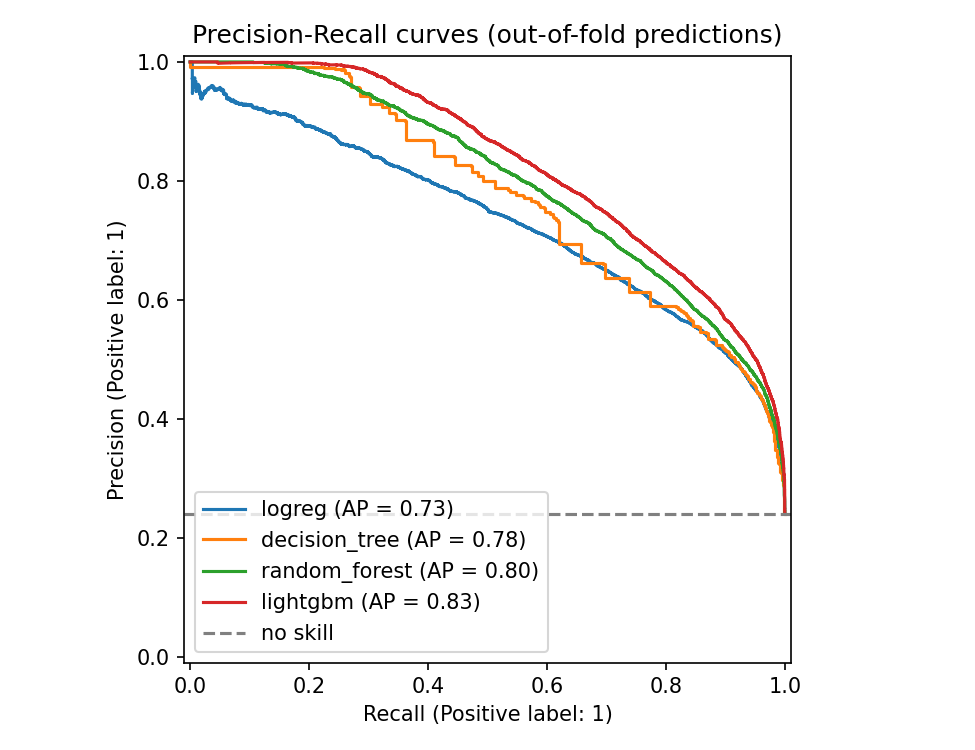
\includegraphics[width=0.62\textwidth]{model_comparison_pr_curves.png}
  \caption{Precision--recall curves of the four models with default hyperparameters, computed from out-of-fold predictions on the development set. The dashed line is the no-skill reference (0.24).}
  \label{fig:pr}
\end{figure}

\paragraph{A note on optimism.}
The best Optuna score is slightly optimistic, because the same folds were used to choose the hyperparameters. Nested cross-validation would remove this bias but costs five times more computation. Like the course, we keep an untouched test set instead: it gives the unbiased final estimate.

% ===========================================================================
\section{Final model and test results}
\label{sec:final}

\paragraph{Choice of the threshold.}
We have no real costs for false positives and false negatives in this problem, so we consider them comparable and choose the threshold that maximises F1 on the out-of-fold predictions of the final LightGBM.
The result is \textbf{0.379}. On the development set, it raises recall from 0.66 to 0.76 and lowers precision from 0.78 to 0.70. If a real cost ratio were known, we would choose the threshold that minimises the expected cost instead.

\paragraph{Test results.}
Table~\ref{tab:test} gives the results of the frozen model on the untouched test set.
The test PR-AUC (0.837) is consistent with the cross-validation estimate ($0.830 \pm 0.007$): the protocol did not produce an optimistic score.
At the tuned threshold, the model finds 74.5\% of high earners, and 71.1\% of the people it flags are really high earners (Figure~\ref{fig:cm_calib}, left: 1{,}742 true positives, 707 false positives and 596 false negatives).

\begin{table}[!htbp]
\centering
\small
\caption{Final LightGBM on the test set (9{,}769 people), used once.}
\label{tab:test}
\begin{tabular}{lccccccc}
\toprule
\textbf{Threshold} & \textbf{PR-AUC} & \textbf{ROC-AUC} & \textbf{Precision} & \textbf{Recall} & \textbf{F1} & \textbf{Accuracy} & \textbf{Brier} \\
\midrule
0.5 (default) & 0.837 & 0.931 & 0.791 & 0.660 & 0.719 & 0.877 & 0.086 \\
\textbf{0.379 (tuned)} & 0.837 & 0.931 & 0.711 & 0.745 & \textbf{0.728} & 0.867 & 0.086 \\
\bottomrule
\end{tabular}
\end{table}

% ===========================================================================
\section{Calibration diagnostics}
\label{sec:calibration}

Good ranking does not guarantee good probabilities. We therefore checked whether a predicted probability of, for example, 30\% really means that about 30\% of these people earn more than \$50K.
We grouped the test predictions into 10 equal-width bins and compared, in each bin, the mean predicted probability with the observed share of positives (Figure~\ref{fig:cm_calib}, right, and Table~\ref{tab:calib}).

\begin{figure}[!htbp]
  \centering
  \begin{subfigure}{0.43\textwidth}
    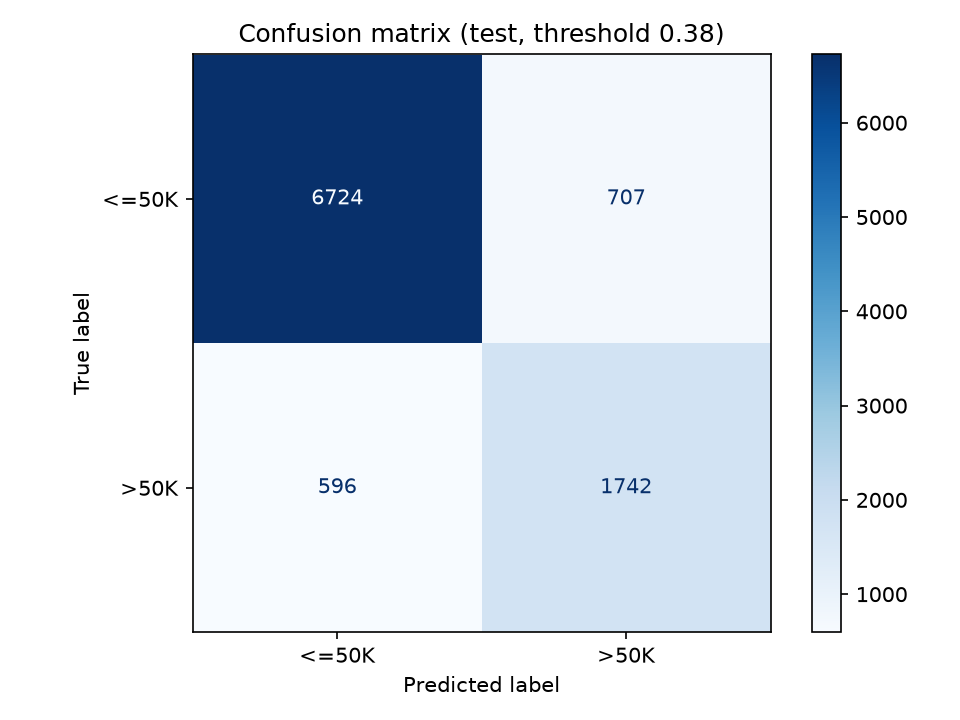
\includegraphics[width=\textwidth]{confusion_matrix.png}
  \end{subfigure}
  \hfill
  \begin{subfigure}{0.48\textwidth}
    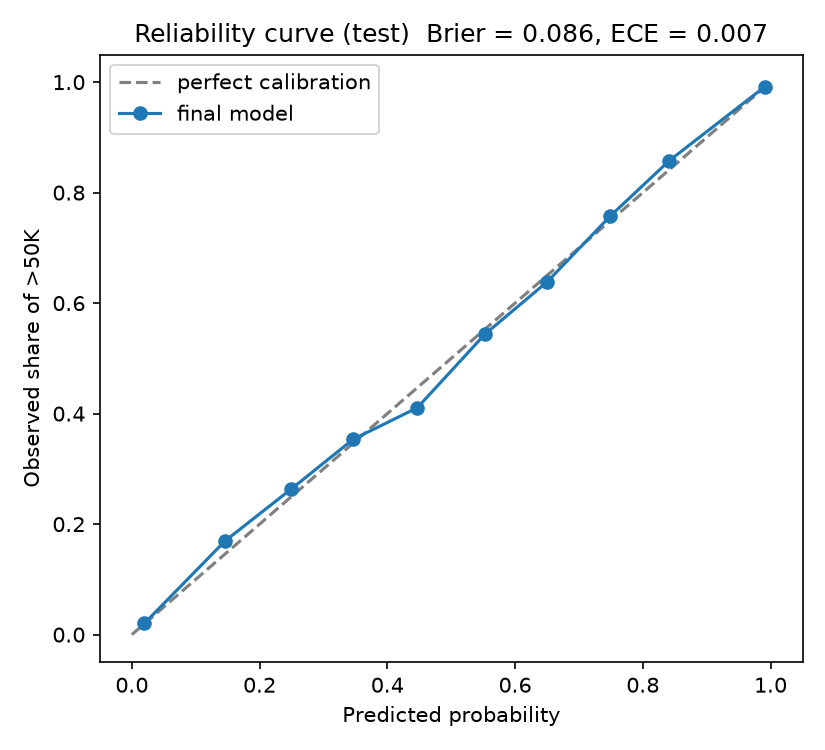
\includegraphics[width=\textwidth]{calibration_curve.png}
  \end{subfigure}
  \caption{Left: confusion matrix on the test set at the tuned threshold. Right: reliability curve on the test set.}
  \label{fig:cm_calib}
\end{figure}

\begin{table}[!htbp]
\centering
\small
\caption{Reliability table on the test set. Gap = predicted $-$ observed (positive: the model over-estimates).}
\label{tab:calib}
\setlength{\tabcolsep}{3pt}\footnotesize\begin{tabular}{lcccccccccc}
\toprule
Mean predicted & 0.019 & 0.146 & 0.250 & 0.347 & 0.447 & 0.553 & 0.650 & 0.749 & 0.841 & 0.991 \\
Observed & 0.020 & 0.169 & 0.264 & 0.354 & 0.411 & 0.544 & 0.639 & 0.757 & 0.858 & 0.991 \\
Gap & $-$0.001 & $-$0.024 & $-$0.014 & $-$0.007 & +0.036 & +0.009 & +0.012 & $-$0.008 & $-$0.016 & $-$0.001 \\
\bottomrule
\end{tabular}
\end{table}

\paragraph{Results.}
The \textbf{Brier score is 0.086} and the \textbf{expected calibration error (ECE) is 0.007}: on average, the predicted probability is less than one percentage point away from the observed frequency.
The curve follows the diagonal closely. The model is neither clearly over-confident nor under-confident: it slightly \emph{under}-estimates the risk in bins 2, 3 and 9 (gaps of $-1.4$ to $-2.4$ points), while bins 1 and 10 are almost perfect, and slightly \emph{over}-estimates it around 0.45 (+3.6 points), which is the largest gap.

\paragraph{Can we trust the probabilities as they are?}
Yes, for a downstream decision on a population similar to the training data. This is also a consequence of our imbalance choice: class weights or resampling would have inflated the probabilities (Brier 0.11 instead of 0.088, Table~\ref{tab:remedies}).
For this reason, we did not apply Platt scaling or isotonic regression: with an ECE below 1 point, there is little to correct, and a recalibration step would add complexity and a risk of overfitting.
Two limits remain. First, the ECE depends on the choice of bins, and we did not report the number of people in each bin; the middle bins contain fewer people, so their gaps are noisier. Second, good overall calibration does not guarantee good calibration in every subgroup; we did not check calibration separately for men and women.

% ===========================================================================
\section{Explainability with SHAP}
\label{sec:shap}

We used SHAP (\texttt{TreeExplainer}) on a random sample of 2{,}000 test rows. A SHAP value tells us how much one feature pushed one prediction up or down, compared with the average prediction. For LightGBM, values are on the log-odds scale: a positive value pushes towards \texttt{>50K}.

\paragraph{Global importance.}
Figure~\ref{fig:shap_global} shows the mean absolute SHAP value and the direction of each effect.
The most important features are \texttt{capital\_net} (0.90), \texttt{age} (0.81), being married (\texttt{Married-civ-spouse}, 0.77), \texttt{education-num} (0.49) and \texttt{hours-per-week} (0.32).
These features make business sense: capital income is a direct sign of wealth, income grows with age and experience, education gives access to better-paid jobs, and full-time work above 40 hours is linked to higher salaries. Being married is also important, probably because in 1994 most high earners in the data were married men (\texttt{relationship\_Husband} is in the top 7).
Our engineered feature \texttt{capital\_net} is the most important feature; its importance comes from capital income itself. We did not test whether the log transformation helps.
\texttt{sex\_Female} is in the top 8 and always lowers the score. The model has learned the gender gap of the data, which is why we audit fairness in Section~\ref{sec:fairness}.

\begin{figure}[!htbp]
  \centering
  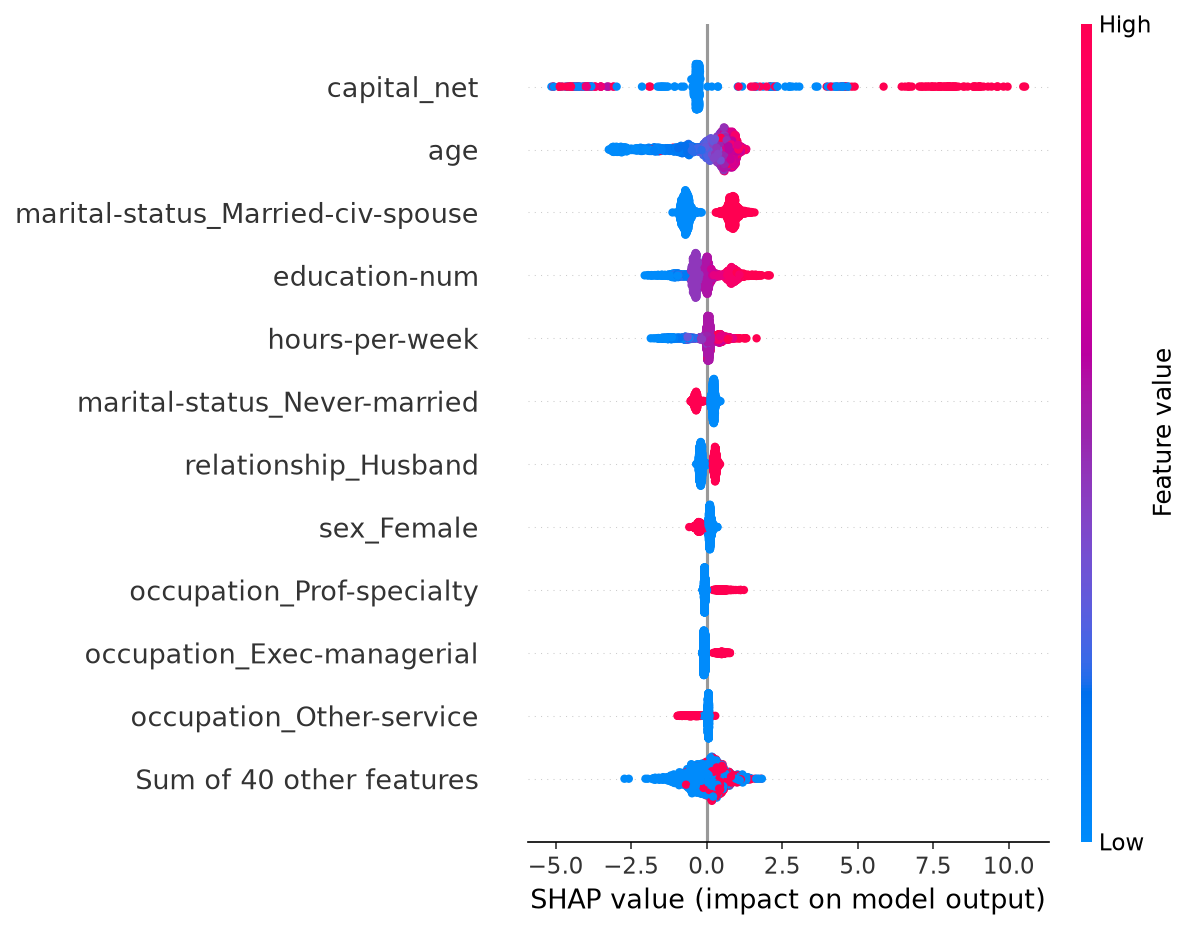
\includegraphics[width=0.66\textwidth]{shap_summary.png}
  \caption{SHAP summary plot (test sample). Each dot is one person; colour = value of the feature (red = high); position = effect on the score.}
  \label{fig:shap_global}
\end{figure}

\paragraph{Local explanations.}
We explained four individual predictions: the most confident true positive, true negative, false positive and false negative. Figure~\ref{fig:shap_local} shows the two errors; the other two are in Appendix~\ref{app:figures}.
\begin{itemize}
  \item \textbf{False positive} (predicted probability 0.91, true label \texttt{<=50K}): this person has a large capital gain (+1.46), is married (+1.06), has 14 years of education (+0.78) and works 50 hours per week. On paper, the profile is very typical of a high earner. The model is wrong for a reasonable reason: the data do not contain the information that would explain the low income.
  \item \textbf{False negative} (predicted probability $\approx$ 0, true label \texttt{>50K}): a 28-year-old person, never married, living with parents (\texttt{Own-child}), working for a state government, with no capital income. Almost every feature lowers the score; only the 13 years of education raise it (+0.65). This is an atypical high earner, young and single, that the model cannot recognise.
\end{itemize}
These two errors show that the model reasons in a sensible way. Its mistakes come from people whose profile is unusual for their income, not from a suspicious feature.
Note that SHAP explains the \emph{model's} behaviour, not the real causes of income.

\begin{figure}[!htbp]
  \centering
  \begin{subfigure}{0.49\textwidth}
    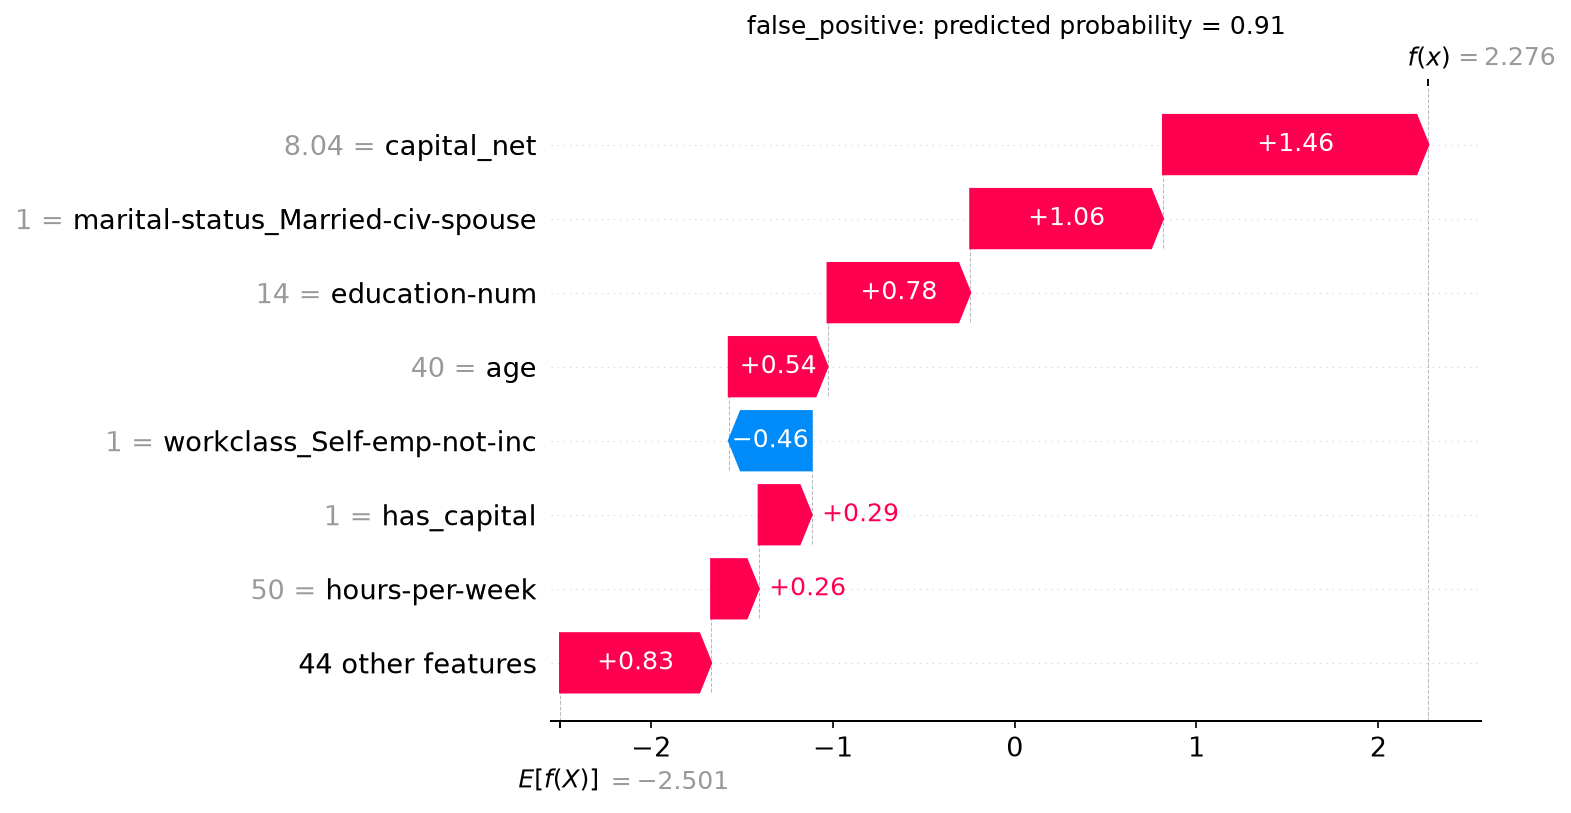
\includegraphics[width=\textwidth]{shap_local_false_positive.png}
  \end{subfigure}
  \hfill
  \begin{subfigure}{0.49\textwidth}
    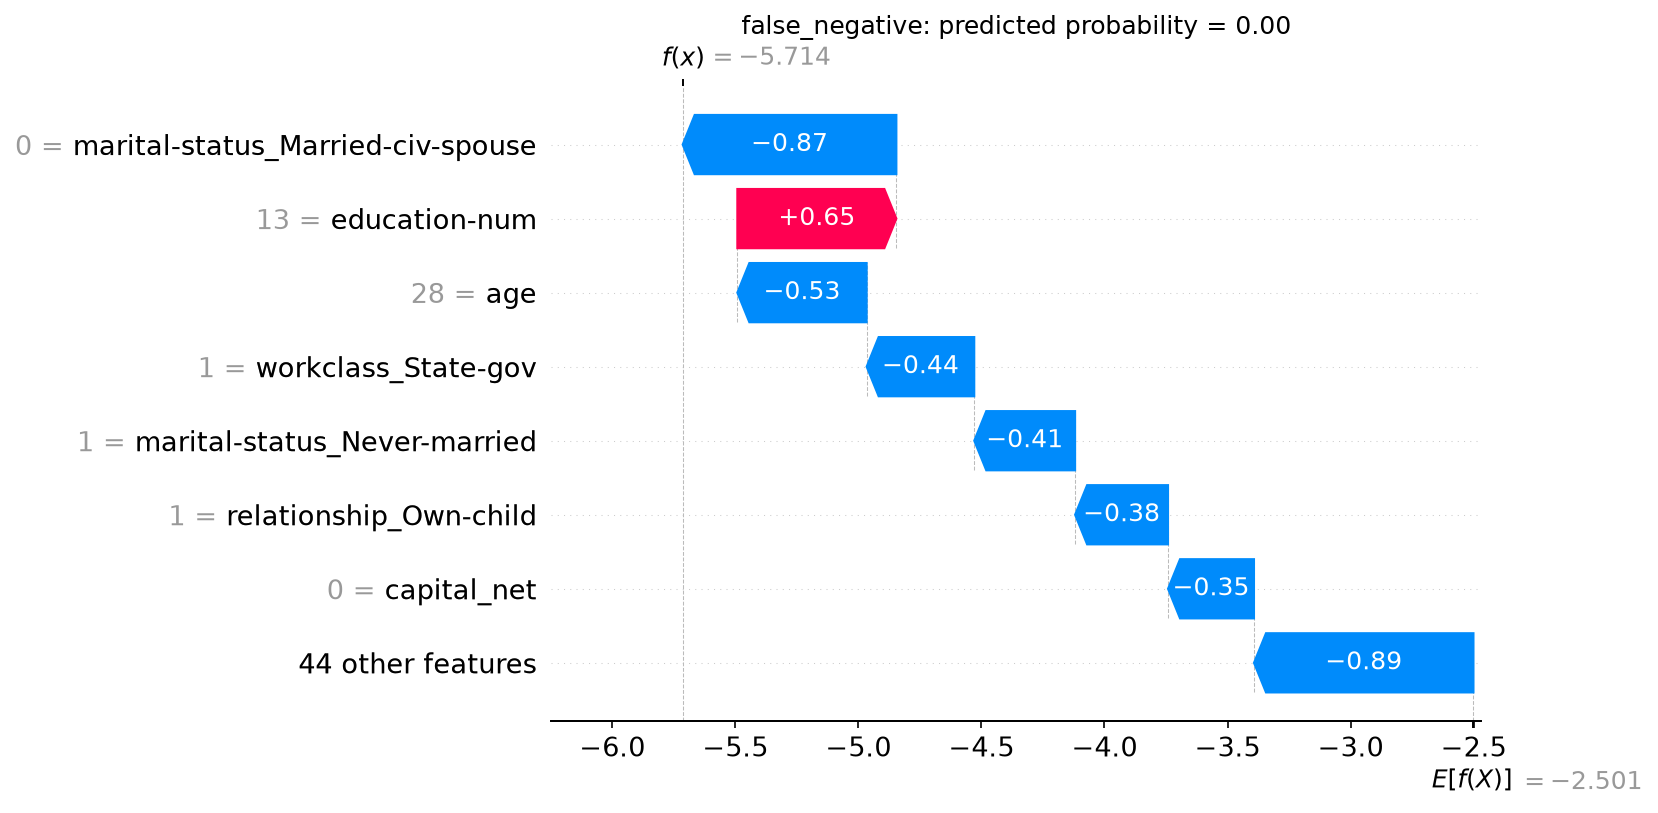
\includegraphics[width=\textwidth]{shap_local_false_negative.png}
  \end{subfigure}
  \caption{SHAP waterfall plots for the most confident false positive (left) and false negative (right). $E[f(X)] = -2.5$ is the average raw score.}
  \label{fig:shap_local}
\end{figure}

% ===========================================================================
\section{Fairness and bias audit}
\label{sec:fairness}

\paragraph{Definition.}
In the data, 30.4\% of men and 10.9\% of women earn more than \$50K. Because these base rates are very different, \emph{demographic parity} (the same share of positive predictions for both groups) would force the model to contradict the labels.
We therefore target \textbf{equal opportunity}: a person who really earns more than \$50K should have the same chance of being detected, whatever their sex. The metric is the gap in recall (true positive rate) between women and men. We also report the demographic parity gap (difference in selection rate) and the false positive rate.

\paragraph{Audit.}
Table~\ref{tab:fair} (top) shows the metrics by sex on the test set with the single threshold 0.379. Each group is large enough for stable estimates (3{,}259 women with 361 high earners, 6{,}510 men with 1{,}977 high earners).
The recall is 68.1\% for women and 75.7\% for men: the model misses high-earning women more often. The \textbf{equal opportunity gap is 7.5 points}. Precision is the same for both groups (0.71).

\paragraph{Mitigation: group-specific thresholds.}
We used a post-processing method: the model is not retrained, but each group receives its own decision threshold.
The thresholds are chosen on the \emph{out-of-fold predictions of the development set}, so that each group reaches the same recall as the single threshold gives overall. The result is \textbf{0.264 for women and 0.395 for men}. They are then applied once to the untouched test set.

\begin{table}[!htbp]
\centering
\small
\caption{Fairness by sex on the test set, before and after mitigation. Base rate = share of real high earners in the group.}
\label{tab:fair}
\setlength{\tabcolsep}{4pt}\begin{tabular}{llccccc}
\toprule
& \textbf{Group} & \textbf{Base rate} & \textbf{Selection rate} & \textbf{Recall (TPR)} & \textbf{FPR} & \textbf{Precision} \\
\midrule
\multirow{2}{*}{Before (threshold 0.379)} & Women & 0.111 & 0.107 & 0.681 & 0.035 & 0.707 \\
 & Men & 0.304 & 0.323 & 0.757 & 0.133 & 0.712 \\
\addlinespace
\multirow{2}{*}{After (0.264 / 0.395)} & Women & 0.111 & 0.133 & 0.751 & 0.056 & 0.626 \\
 & Men & 0.304 & 0.315 & 0.748 & 0.127 & 0.720 \\
\bottomrule
\end{tabular}

\vspace{6pt}
\begin{tabular}{lccc}
\toprule
\textbf{Test set} & \textbf{Before} & \textbf{After} & \textbf{Change} \\
\midrule
Equal opportunity gap (recall) & 0.075 & \textbf{0.003} & $-$0.072 \\
Demographic parity gap (selection rate) & 0.216 & 0.182 & $-$0.034 \\
Overall precision & 0.711 & 0.704 & $-$0.008 \\
Overall recall & 0.745 & 0.748 & +0.003 \\
Overall F1 & 0.728 & 0.725 & $-$0.003 \\
\bottomrule
\end{tabular}
\end{table}

\begin{figure}[!htbp]
  \centering
  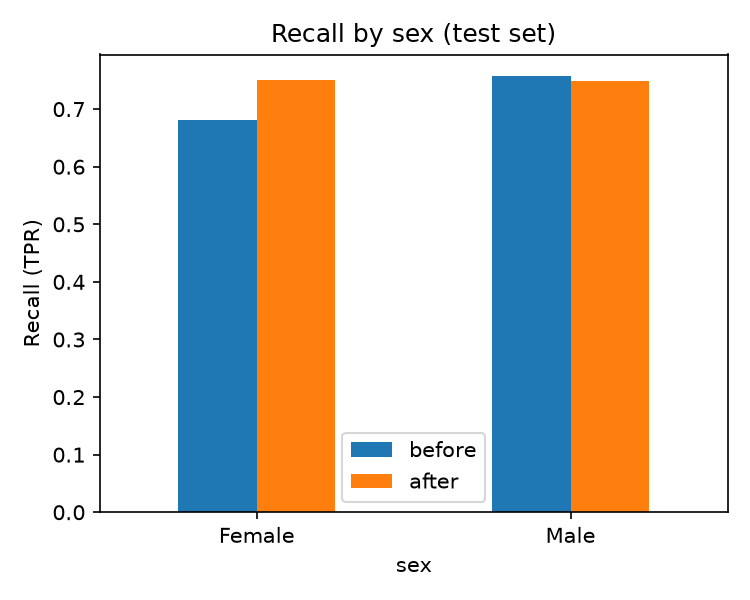
\includegraphics[width=0.45\textwidth]{fairness_recall_by_sex.png}
  \caption{Recall by sex on the test set, before and after mitigation.}
  \label{fig:fair}
\end{figure}

\paragraph{Discussion.}
Before mitigation, the recall gap is 7.5 points, with a 95\% bootstrap confidence interval of 2.1 to 12.9 points (2{,}000 resamples of the test set): the gap is real. After mitigation, the gap is 0.3 points, but with only 361 high-earning women in the test set its interval goes from $-5.2$ to $+4.6$ points: the remaining gap is not statistically distinguishable from zero. The overall F1 only loses 0.003. It works on the untouched test set, so the result is not a product of overfitting.
There is a price. To catch more high-earning women, the model also flags more women by mistake: their false positive rate goes from 3.5\% to 5.6\% and the precision of their alerts drops from 0.71 to 0.63. The demographic parity gap stays large (0.18), which is expected because the base rates are different.
The method also needs to know the sex of each person at decision time. In some contexts (credit, hiring), using a protected attribute explicitly in the decision rule may be illegal, even if the goal is to reduce bias.
Finally, simply removing \texttt{sex} from the features would not be a good alternative: \texttt{relationship} (\emph{Husband}/\emph{Wife}) reveals it almost perfectly, so the model would still learn the same gap.

% ===========================================================================
\section{Limitations and conclusion}
\label{sec:conclusion}

\paragraph{Limitations.}
\begin{itemize}
  \item \textbf{Old data:} The census dates from 1994 and the \$50K threshold is not adjusted for inflation. The model should not be used on today's population without new data; a distribution shift would also break the calibration.
  \item \textbf{Threshold choice:} We maximised F1 because we have no real costs. A real application should use its own cost ratio.
  \item \textbf{Diagnostics:} We audited the model by sex only. A slice analysis by race, age group or occupation could reveal other weak groups. Calibration by group and the number of people per calibration bin were not reported.
  \item \textbf{Explainability:} SHAP describes the model, not causes. Permutation importance or partial dependence plots would complete the picture.
  \item \textbf{Tuning budget:} We used 15 Optuna trials per model to keep the training time around 5 minutes. A larger budget might add a little performance to the tree-based models. In particular, the best LightGBM uses 600 trees and the best decision tree a depth of 20: both values are at the upper limit of our search space, so the optimum may lie beyond it.
\end{itemize}

\paragraph{Conclusion.}
We built a complete and leakage-free pipeline for the Adult dataset. LightGBM is the best of the four models (test PR-AUC 0.837, F1 0.728 at a tuned threshold). Its probabilities are well calibrated (ECE 0.007), its main features make business sense, and a simple post-processing step closes the recall gap between men and women (7.5 points before, not statistically different from zero after) for a very small loss in performance.
Our main methodological lesson is that the simplest remedy was the best one: tuning the decision threshold handled the class imbalance as well as reweighting or resampling, while keeping trustworthy probabilities.

% ===========================================================================
\section*{Use of AI assistants}
\addcontentsline{toc}{section}{Use of AI assistants}
We used an AI assistant to help us during the whole project. We chose the structure of the repository among options proposed by the assistant, and it helped us write the first version of all Python scripts, and helped us draft this report from our results. We chose the dataset and the four models, ran all the code on our own computers, reviewed and simplified the code, checked every number in this report against the files produced by our runs, and wrote and checked the interpretations.

\section*{Contribution statement}
\addcontentsline{toc}{section}{Contribution statement}

\begin{table}[H]
\centering
\small
\begin{tabular}{lp{11cm}}
\toprule
\textbf{Member} & \textbf{Contribution} \\
\midrule
Alexandre Casagranda & Creation of the first code (\texttt{prepare.py} and \texttt{eda.py}) and analysis. \\
Simon Mazabraud & Analysis and code of \texttt{train.py}. \\
Ryan Khlaief & Analysis and code of \texttt{evaluate.py}. \\
\bottomrule
\end{tabular}
\end{table}

% ===========================================================================
\newpage
\appendix

\section{Run log of all tuning trials}
\label{app:runlog}

The complete run log is the file \texttt{reports/run\_log.csv} in the repository. It also contains the imbalance experiments and the default-parameter comparison. The table below lists the 60 Optuna trials (15 per model). The metric is the mean (and standard deviation) of PR-AUC over the 5 folds. The best trial of each model is shaded; its artifact is the refitted model. The artifact of the other trials is the optimisation plot of the model (Appendix~\ref{app:figures}).

{\scriptsize
\setlength{\tabcolsep}{3pt}\begin{longtable}{lp{6.9cm}ccl}
\toprule
\textbf{Trial} & \textbf{Parameters} & \textbf{CV PR-AUC} & \textbf{Std} & \textbf{Artifact} \\
\endfirsthead
\toprule
\textbf{Trial} & \textbf{Parameters} & \textbf{CV PR-AUC} & \textbf{Std} & \textbf{Artifact} \\
\midrule
\endhead
\bottomrule
\endfoot
\midrule
\multicolumn{5}{l}{\textbf{Logistic regression}}\\
00 & C=0.0746 & 0.7346 & 0.0113 & \texttt{figures/optuna\_logreg.png}\\
01 & C=56.7 & 0.7347 & 0.0110 & \texttt{figures/optuna\_logreg.png}\\
02 & C=4.57 & 0.7347 & 0.0111 & \texttt{figures/optuna\_logreg.png}\\
03 & C=0.985 & 0.7348 & 0.0111 & \texttt{figures/optuna\_logreg.png}\\
04 & C=0.00603 & 0.7282 & 0.0112 & \texttt{figures/optuna\_logreg.png}\\
05 & C=0.00603 & 0.7282 & 0.0112 & \texttt{figures/optuna\_logreg.png}\\
06 & C=0.00195 & 0.7164 & 0.0110 & \texttt{figures/optuna\_logreg.png}\\
07 & C=21.4 & 0.7348 & 0.0111 & \texttt{figures/optuna\_logreg.png}\\
08 & C=1.01 & 0.7348 & 0.0111 & \texttt{figures/optuna\_logreg.png}\\
09 & C=3.47 & 0.7347 & 0.0112 & \texttt{figures/optuna\_logreg.png}\\
10 & C=0.239 & 0.7348 & 0.0112 & \texttt{figures/optuna\_logreg.png}\\
11 & C=0.205 & 0.7348 & 0.0112 & \texttt{figures/optuna\_logreg.png}\\
12 & C=0.0841 & 0.7347 & 0.0113 & \texttt{figures/optuna\_logreg.png}\\
13 & C=0.0993 & 0.7347 & 0.0113 & \texttt{figures/optuna\_logreg.png}\\
\rowcolor{gray!15} 14 & C=0.236 & 0.7348 & 0.0113 & \texttt{models/logreg\_tuned.joblib}\\
\midrule
\multicolumn{5}{l}{\textbf{Decision tree}}\\
00 & depth=9, min\_leaf=166 & 0.7641 & 0.0113 & \texttt{figures/optuna\_decision\_tree.png}\\
01 & depth=16, min\_leaf=44 & 0.7864 & 0.0113 & \texttt{figures/optuna\_decision\_tree.png}\\
02 & depth=5, min\_leaf=8 & 0.7021 & 0.0116 & \texttt{figures/optuna\_decision\_tree.png}\\
03 & depth=4, min\_leaf=121 & 0.6747 & 0.0097 & \texttt{figures/optuna\_decision\_tree.png}\\
04 & depth=13, min\_leaf=66 & 0.7868 & 0.0111 & \texttt{figures/optuna\_decision\_tree.png}\\
05 & depth=3, min\_leaf=179 & 0.6413 & 0.0103 & \texttt{figures/optuna\_decision\_tree.png}\\
06 & depth=17, min\_leaf=10 & 0.7666 & 0.0042 & \texttt{figures/optuna\_decision\_tree.png}\\
07 & depth=6, min\_leaf=9 & 0.7300 & 0.0134 & \texttt{figures/optuna\_decision\_tree.png}\\
08 & depth=8, min\_leaf=33 & 0.7592 & 0.0144 & \texttt{figures/optuna\_decision\_tree.png}\\
09 & depth=10, min\_leaf=14 & 0.7768 & 0.0105 & \texttt{figures/optuna\_decision\_tree.png}\\
10 & depth=15, min\_leaf=191 & 0.7731 & 0.0090 & \texttt{figures/optuna\_decision\_tree.png}\\
11 & depth=16, min\_leaf=35 & 0.7861 & 0.0096 & \texttt{figures/optuna\_decision\_tree.png}\\
12 & depth=13, min\_leaf=86 & 0.7826 & 0.0109 & \texttt{figures/optuna\_decision\_tree.png}\\
\rowcolor{gray!15} 13 & depth=20, min\_leaf=73 & 0.7887 & 0.0117 & \texttt{models/decision\_tree\_tuned.joblib}\\
14 & depth=20, min\_leaf=94 & 0.7831 & 0.0108 & \texttt{figures/optuna\_decision\_tree.png}\\
\midrule
\multicolumn{5}{l}{\textbf{Random forest (200 trees)}}\\
00 & depth=15, min\_leaf=20, max\_feat=sqrt & 0.7916 & 0.0094 & \texttt{figures/optuna\_random\_forest.png}\\
01 & depth=9, min\_leaf=4, max\_feat=0.5 & 0.8069 & 0.0080 & \texttt{figures/optuna\_random\_forest.png}\\
02 & depth=21, min\_leaf=15, max\_feat=0.5 & 0.8081 & 0.0087 & \texttt{figures/optuna\_random\_forest.png}\\
03 & depth=26, min\_leaf=5, max\_feat=0.5 & 0.8068 & 0.0084 & \texttt{figures/optuna\_random\_forest.png}\\
04 & depth=13, min\_leaf=11, max\_feat=sqrt & 0.7943 & 0.0091 & \texttt{figures/optuna\_random\_forest.png}\\
05 & depth=21, min\_leaf=3, max\_feat=0.5 & 0.8064 & 0.0081 & \texttt{figures/optuna\_random\_forest.png}\\
06 & depth=17, min\_leaf=16, max\_feat=0.5 & 0.8082 & 0.0088 & \texttt{figures/optuna\_random\_forest.png}\\
07 & depth=20, min\_leaf=1, max\_feat=sqrt & 0.7953 & 0.0084 & \texttt{figures/optuna\_random\_forest.png}\\
08 & depth=7, min\_leaf=19, max\_feat=sqrt & 0.7750 & 0.0089 & \texttt{figures/optuna\_random\_forest.png}\\
09 & depth=13, min\_leaf=2, max\_feat=sqrt & 0.7993 & 0.0090 & \texttt{figures/optuna\_random\_forest.png}\\
10 & depth=11, min\_leaf=11, max\_feat=0.5 & 0.8087 & 0.0083 & \texttt{figures/optuna\_random\_forest.png}\\
11 & depth=8, min\_leaf=11, max\_feat=0.5 & 0.8024 & 0.0082 & \texttt{figures/optuna\_random\_forest.png}\\
12 & depth=14, min\_leaf=15, max\_feat=0.5 & 0.8084 & 0.0085 & \texttt{figures/optuna\_random\_forest.png}\\
\rowcolor{gray!15} 13 & depth=14, min\_leaf=8, max\_feat=0.5 & 0.8105 & 0.0082 & \texttt{models/random\_forest\_tuned.joblib}\\
14 & depth=12, min\_leaf=11, max\_feat=0.5 & 0.8092 & 0.0086 & \texttt{figures/optuna\_random\_forest.png}\\
\midrule
\multicolumn{5}{l}{\textbf{LightGBM}}\\
00 & n\_est=300, lr=0.173, leaves=36, min\_child=62, colsample=0.578 & 0.8222 & 0.0071 & \texttt{figures/optuna\_lightgbm.png}\\
01 & n\_est=150, lr=0.0119, leaves=48, min\_child=62, colsample=0.854 & 0.8114 & 0.0081 & \texttt{figures/optuna\_lightgbm.png}\\
02 & n\_est=100, lr=0.183, leaves=45, min\_child=25, colsample=0.591 & 0.8279 & 0.0065 & \texttt{figures/optuna\_lightgbm.png}\\
03 & n\_est=200, lr=0.0249, leaves=23, min\_child=46, colsample=0.646 & 0.8224 & 0.0077 & \texttt{figures/optuna\_lightgbm.png}\\
04 & n\_est=400, lr=0.0152, leaves=14, min\_child=40, colsample=0.728 & 0.8217 & 0.0080 & \texttt{figures/optuna\_lightgbm.png}\\
05 & n\_est=500, lr=0.0182, leaves=23, min\_child=61, colsample=0.523 & 0.8281 & 0.0072 & \texttt{figures/optuna\_lightgbm.png}\\
06 & n\_est=400, lr=0.0167, leaves=9, min\_child=96, colsample=0.983 & 0.8132 & 0.0083 & \texttt{figures/optuna\_lightgbm.png}\\
07 & n\_est=500, lr=0.0249, leaves=9, min\_child=70, colsample=0.72 & 0.8237 & 0.0072 & \texttt{figures/optuna\_lightgbm.png}\\
08 & n\_est=150, lr=0.0441, leaves=8, min\_child=92, colsample=0.629 & 0.8124 & 0.0082 & \texttt{figures/optuna\_lightgbm.png}\\
09 & n\_est=450, lr=0.0254, leaves=23, min\_child=57, colsample=0.592 & 0.8295 & 0.0070 & \texttt{figures/optuna\_lightgbm.png}\\
10 & n\_est=450, lr=0.131, leaves=20, min\_child=14, colsample=0.521 & 0.8279 & 0.0065 & \texttt{figures/optuna\_lightgbm.png}\\
11 & n\_est=400, lr=0.0218, leaves=30, min\_child=79, colsample=0.505 & 0.8282 & 0.0071 & \texttt{figures/optuna\_lightgbm.png}\\
12 & n\_est=350, lr=0.0225, leaves=27, min\_child=94, colsample=0.541 & 0.8273 & 0.0072 & \texttt{figures/optuna\_lightgbm.png}\\
13 & n\_est=550, lr=0.026, leaves=41, min\_child=85, colsample=0.517 & 0.8301 & 0.0071 & \texttt{figures/optuna\_lightgbm.png}\\
\rowcolor{gray!15} 14 & n\_est=600, lr=0.0421, leaves=29, min\_child=71, colsample=0.536 & 0.8301 & 0.0069 & \texttt{models/lightgbm\_tuned.joblib}\\
\end{longtable}
}

\section{Additional figures}
\label{app:figures}

\begin{figure}[!htbp]
  \centering
  \begin{subfigure}{0.49\textwidth}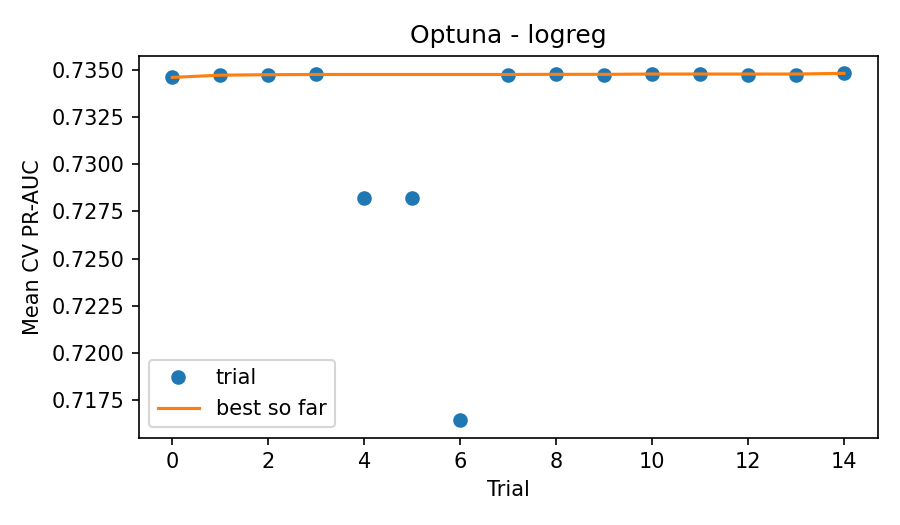
\includegraphics[width=\textwidth]{optuna_logreg.png}\end{subfigure}
  \hfill
  \begin{subfigure}{0.49\textwidth}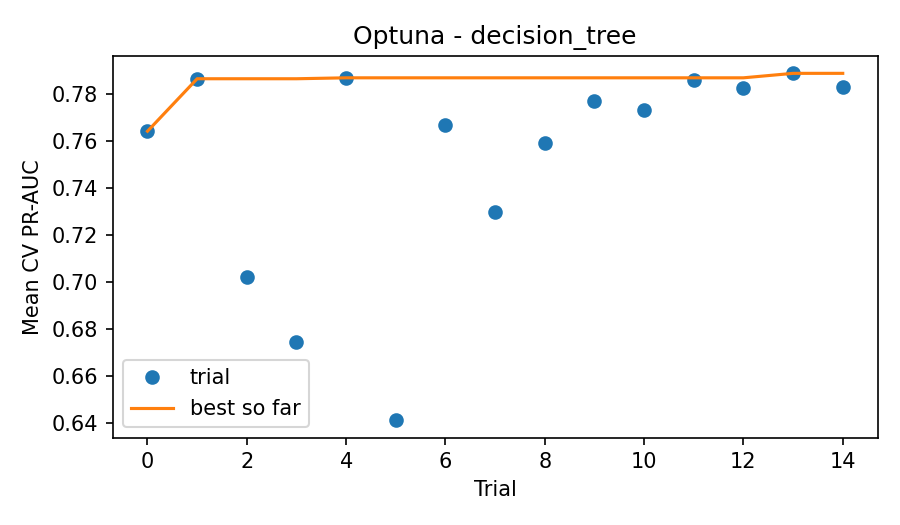
\includegraphics[width=\textwidth]{optuna_decision_tree.png}\end{subfigure}\\[4pt]
  \begin{subfigure}{0.49\textwidth}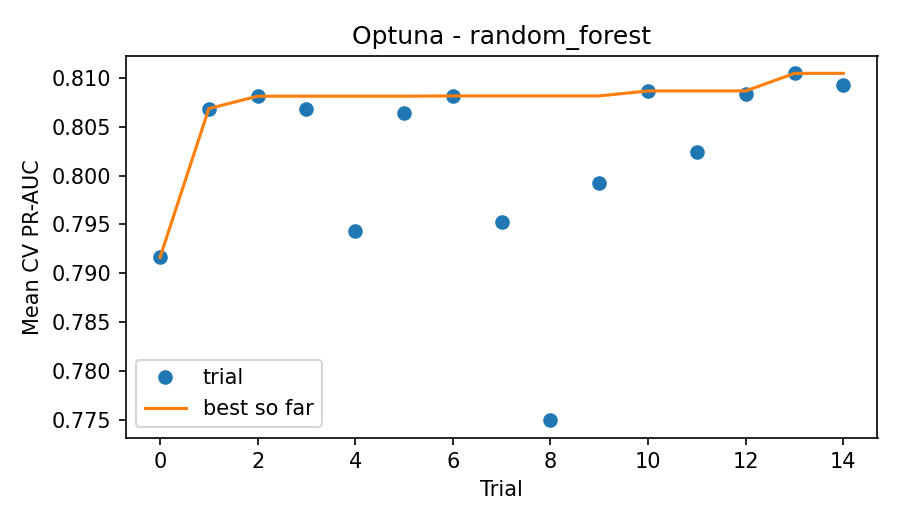
\includegraphics[width=\textwidth]{optuna_random_forest.png}\end{subfigure}
  \hfill
  \begin{subfigure}{0.49\textwidth}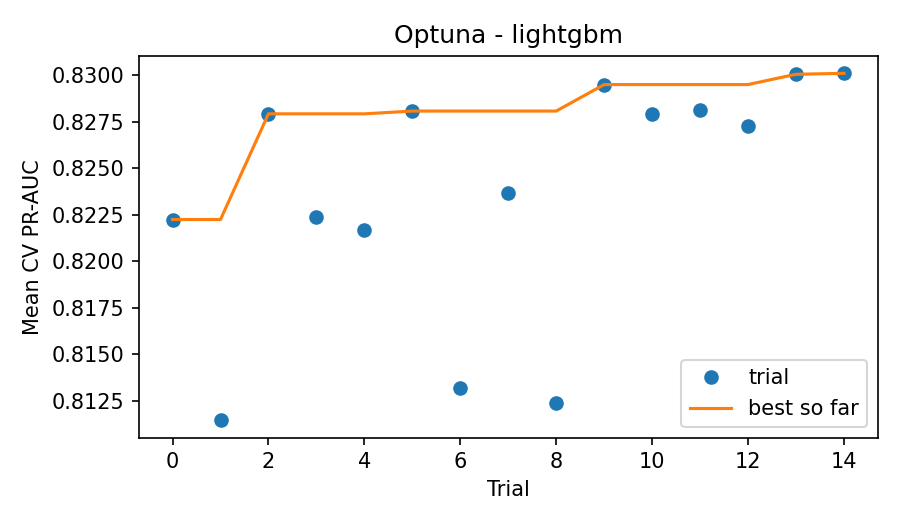
\includegraphics[width=\textwidth]{optuna_lightgbm.png}\end{subfigure}
  \caption{Optuna optimisation history of the four models (mean CV PR-AUC of each trial and best value so far).}
\end{figure}

\begin{figure}[!htbp]
  \centering
  \begin{subfigure}{0.49\textwidth}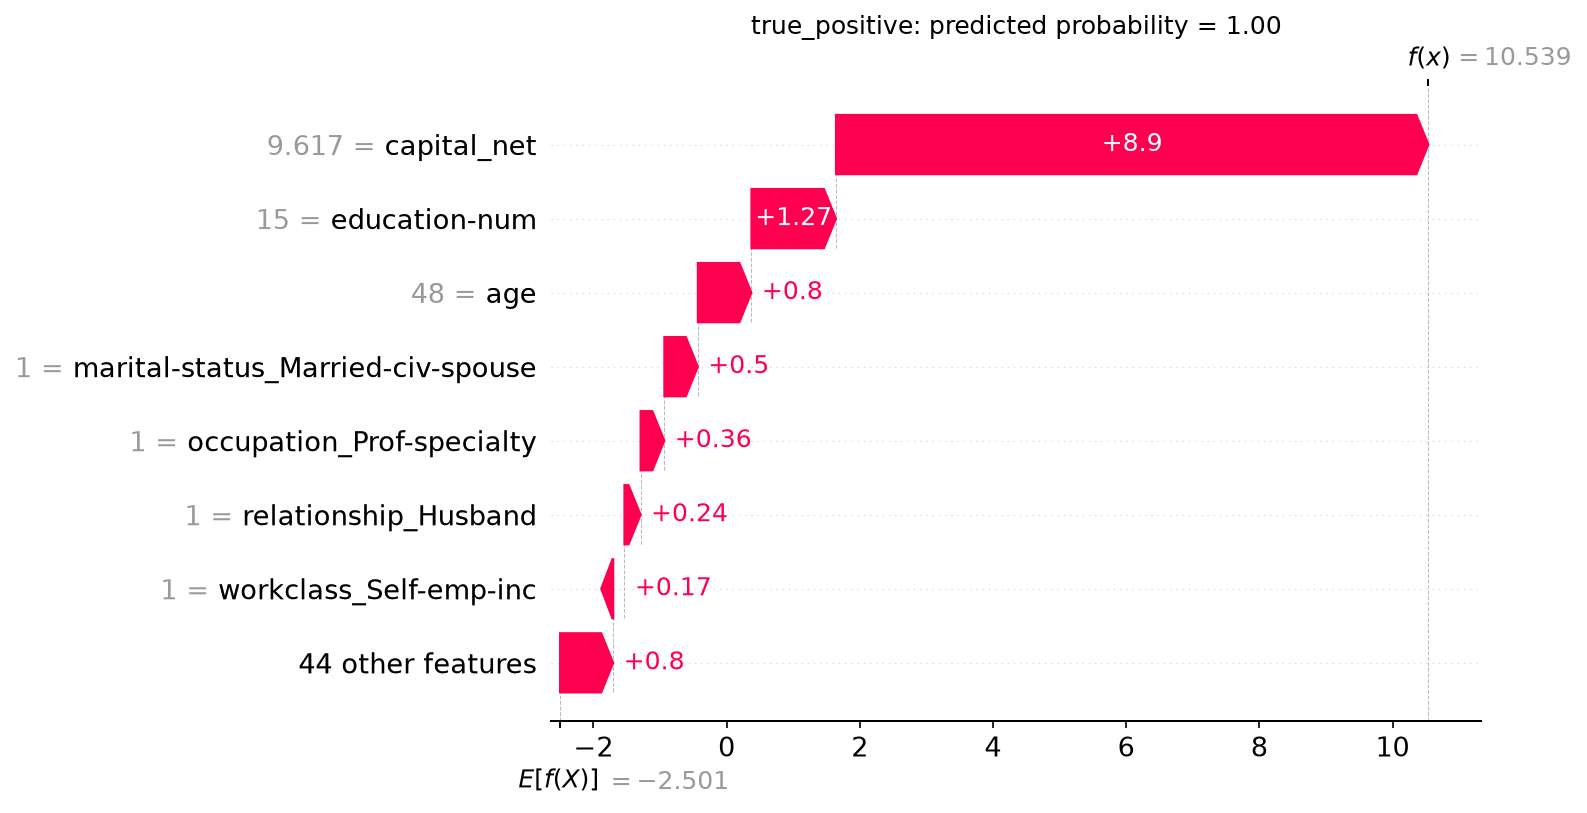
\includegraphics[width=\textwidth]{shap_local_true_positive.png}\end{subfigure}
  \hfill
  \begin{subfigure}{0.49\textwidth}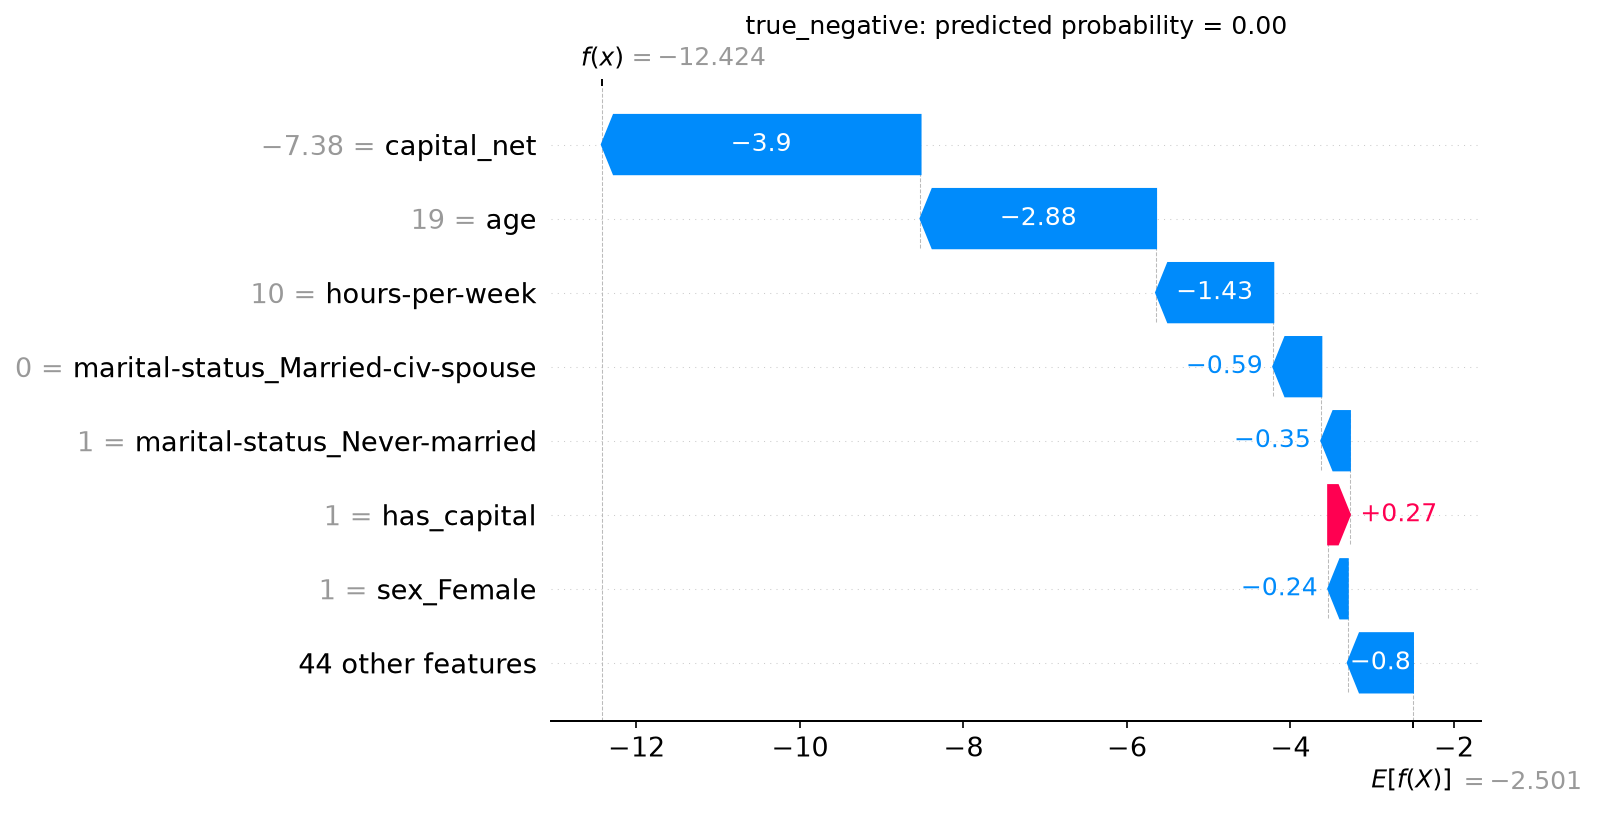
\includegraphics[width=\textwidth]{shap_local_true_negative.png}\end{subfigure}
  \caption{SHAP waterfall plots for the most confident true positive (left) and true negative (right).}
\end{figure}

\begin{figure}[!htbp]
  \centering
  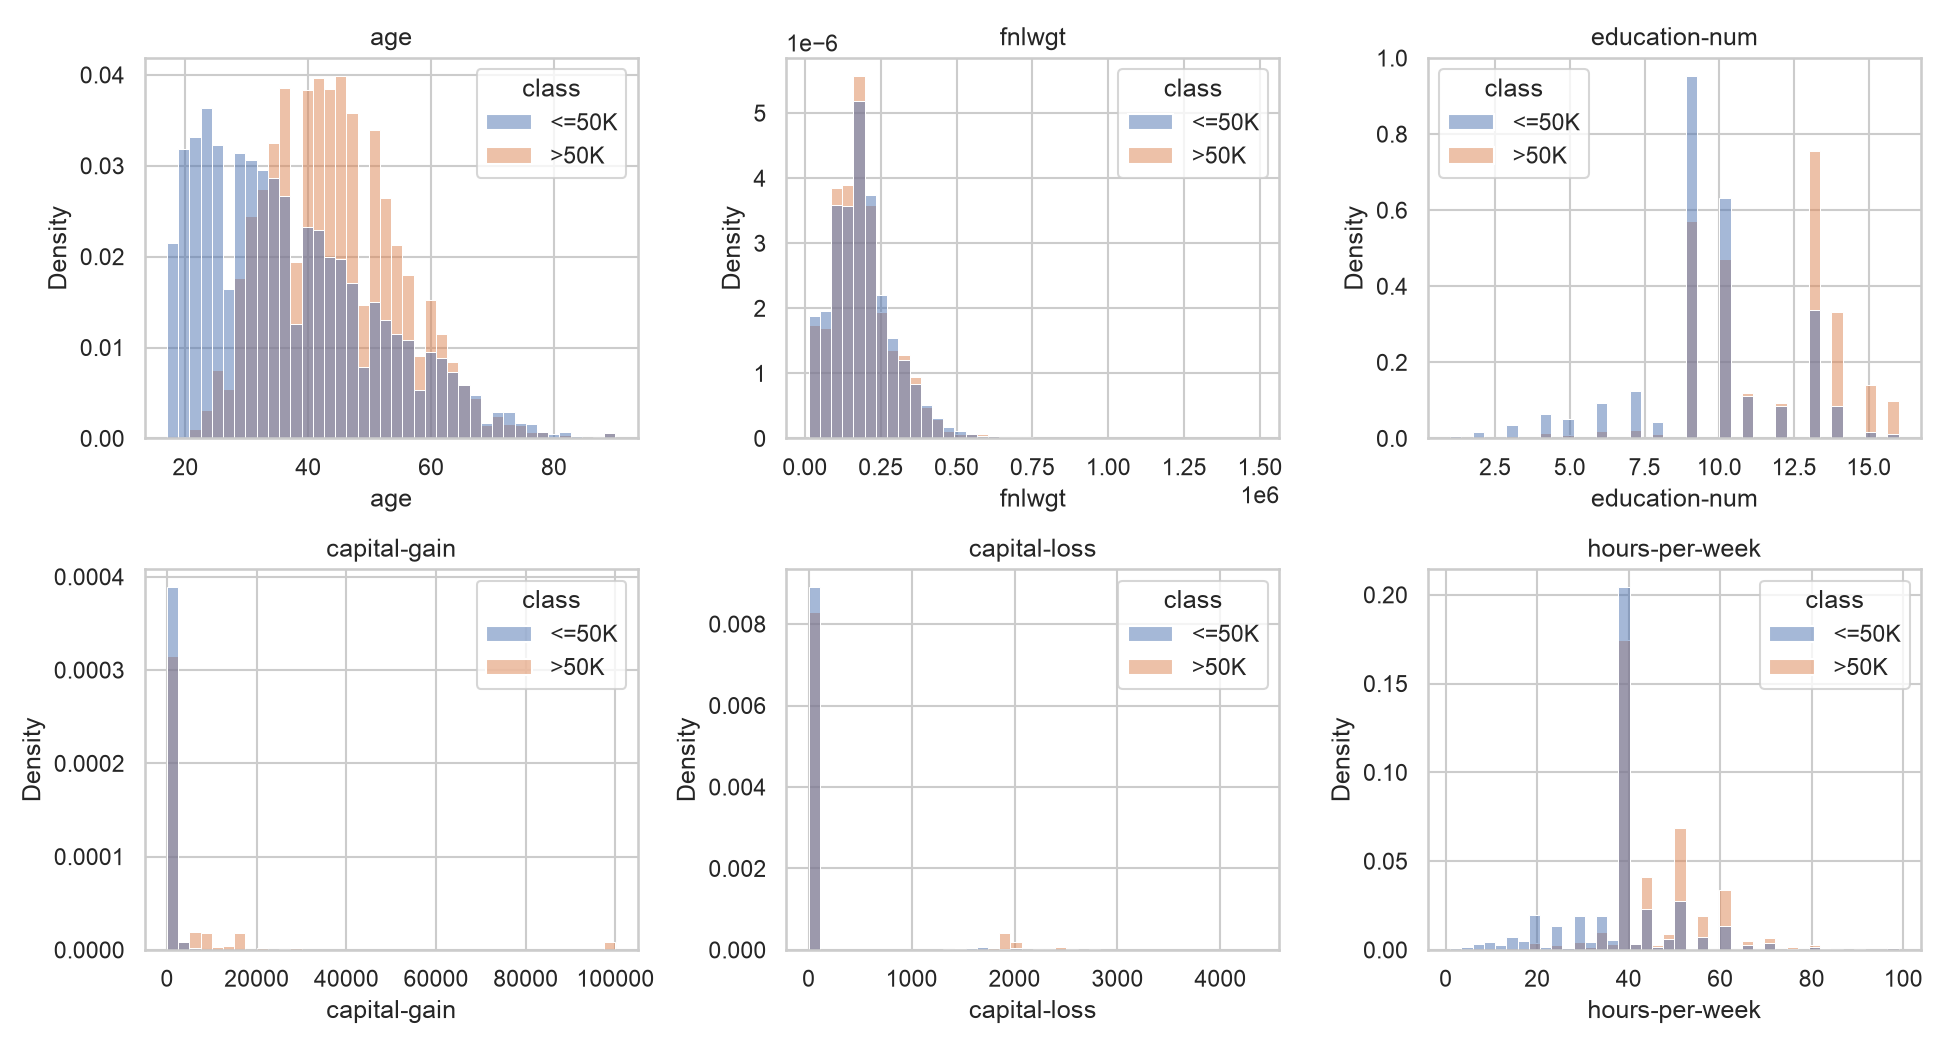
\includegraphics[width=0.85\textwidth]{eda_numeric_distributions.png}
  \caption{Distribution of the numeric features by class (densities).}
\end{figure}

\end{document}
